\documentclass{./../Latex/handout}
\begin{document}
\thispagestyle{plain}
\myheader{Optimization}

Optimization is the process of finding the best solution to a problem, given a set of constraints and objectives. In economics, optimization plays a central role in understanding how individuals, firms, and governments make decisions to allocate scarce resources efficiently. In the context of functions, optimization involves finding a function's maximum or minimum value. 

\vspace{-1em}
%%%%%%%%%%%%% Global vs. Local Extrema
\subsection*{Global vs. Local Extrema}
\begin{itemize}
  \item Local maximum: A point where the function attains its \textit{highest} value within a neighborhood. 
 \item Local minimum: A point where the function attains its \textit{lowest} value within a neighborhood.
 \item Global (or absolute) maximum: A point where the function attains its \textit{highest} value over the entire domain.
 \item Global (or absolute) minimum: A point where the function attains its \textit{lowest} value over the entire domain.
 \end{itemize}
 
 % FIGURE: Global vs local
\begin{center}
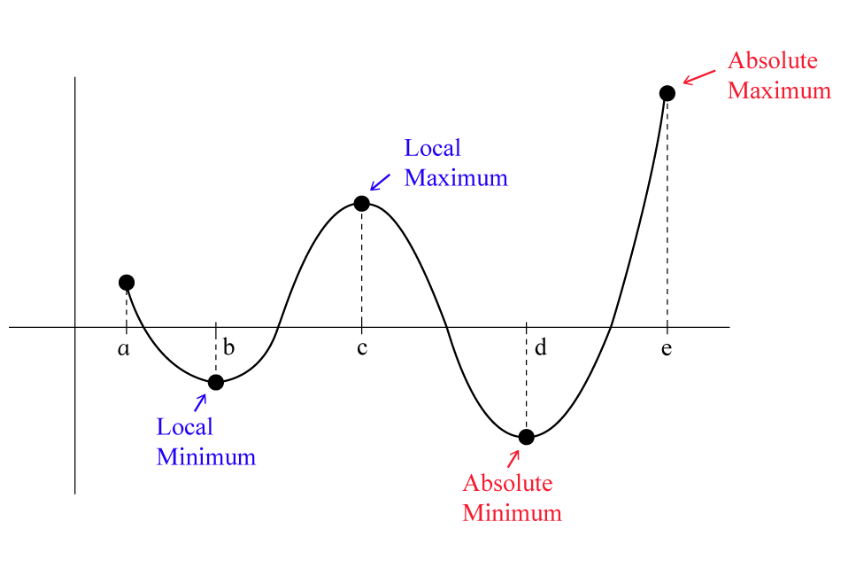
\includegraphics[scale=0.4]{./Input/global_vs_local.png}	\\
\end{center} 

Note that all global extrema are also considered local extrema. Furthermore, there can be multiple local and global extrema for a function. For example, consider the constant function $f(x) = 2$. In this case, all points in the function's domain are global maxima and global minima. There are also functions that have no extremum points, such as $f(x)=x$, which continuously increases as $x$ increases and continuously decreases as $x$ decreases, without reaching any peak or valley.

%%%%%%%%%%%%%%%%%%%%%%%%%%%%%%%%%%%%%%%%%%%%%%%%%%%%%%%%%%
% Unconstrained Optimization with One Variable
%%%%%%%%%%%%%%%%%%%%%%%%%%%%%%%%%%%%%%%%%%%%%%%%%%%%%%%%%%

\section{Unconstrained Optimization with One Variable}

We will start with the simple case of finding a maximum or a minimum of a single-variable function.  First, we will cover the first and second-order conditions for identifying the local maxima or minima of a function. We will then briefly discuss the conditions necessary for identifying global extrema.

%%%%%%%%%%%% First and Second-Order Conditions

\subsection{First and Second-Order Conditions}
 
As illustrated in the figure above, our objective is to locate the peaks or valleys of a function.  Since the derivative captures the rate of change of a function, the derivative of the function at peaks and valleys should be equal to zero. This is because the function is relatively flat in the small neighborhood of the peak or valley. 

We define a critical point as a point where the function's derivative is equal to zero. All local maxima and minima of a function, if any, must occur at critical points where the derivative of the function is equal to zero. \\

% BOX: Critical point
\fbox{\begin{minipage}{\textwidth}
The \textit{necessary} condition for $x^*$ to be a maximum or minimum point of a continuously differentiable function $f(x)$ is: \\
$$f'(x^*) = 0$$ 

Here, $x^*$ is called a critical/stationary point. 
\end{minipage}}\\

\noindent\textit{Example.} Let's find all the critical points for the function $f(x) = x^2 -24 x + 36 $. \\
We start by taking the derivative of $f(x)$: $$f'(x) = 2x-24$$
Next, we set $f'(x)$ equal to zero and solve for $x$. $2x-24=0 \rightarrow x =12$. Therefore, the critical point of $f(x)$ is $x^* = 12$.   \\

Note that it is necessary that at any maxima or minima, the derivative of the function is 0. To see this, consider a point $c$ where $f'(c)>0$, so the function is increasing at point $c$. Then the value of the function at a point just to the left of $c$ will be smaller than $f(c)$, so $c$ cannot be a local minimum. Similarly, the value of the function at a point just to the right of $c$ will be greater than $f(c)$, so $c$ cannot be a local maximum. 

While being a critical point is a necessary condition, it is not a sufficient condition for maxima or minima. This means that at any maximum or minimum point, the derivative of the function must be equal to zero. However, simply having a zero derivative at a point is not enough to conclude that the point is a maximum or a minimum. In some cases, the function may have an \textit{inflection} point or a flat spot, as shown in the following figure.

% FIGURE: Inflection point
\begin{center}
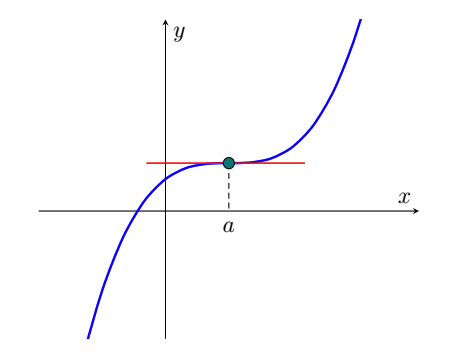
\includegraphics[scale=0.55]{./Input/inflection.png} \\
\end{center} 

Furthermore, even if we have identified a critical point that is not an inflection point, we still cannot tell whether it is a maximum or a minimum point. To determine whether the point is indeed a maximum, a minimum, or neither, we need to analyze the behavior of the function in the neighborhood of the critical point. For instance, when we are at a peak, it should be the case that the function was increasing on the left side of the critical point $x^*$ and decreasing on the right side. In other words, the derivative of the function was positive on the left side of $x^*$ and negative on the right side. This approach is called the first derivative test. \\

% BOX: First Derivative Test
\fbox{\begin{minipage}{\textwidth}
\textit{First Derivative Test} \\~\\
Suppose $f^{\prime}\left(x_{0}\right)=0$, then $x^*$ is a 
\begin{itemize}
  \item maximum if $f^{\prime}(x)$ goes from $+$ to $-$ in the immediate neighborhood of $x_{0}$ 
  \item minimum if $f^{\prime}(x)$ goes from $-$ to $+$ in the immediate neighborhood of $x_{0}$ 
  \item not an extreme point if $f^{\prime}(x)$ has the same sign in the immediate neighborhood of $x_{0}$
\end{itemize}
\end{minipage}}\\

% FIGURE: First Derivative Test
\begin{center}
\begin{tikzpicture}[scale=1.35, transform shape]
\begin{axis}[axis lines = center, ymax=3, xtick, ytick, ymin=-2, xmin=-35, xmax=65]
\addplot [domain=-30:60, samples=100, line width = 0.3mm]
{cos(5*x+2)+cos(2*x+2)};
\draw[dashed,red] (250,400) -- (450,400) node[above, yshift=-2, xshift=0] {\scriptsize $f'(x)=0$};
\draw[dashed,red] (650,120) -- (850,120)node[above, yshift=-20, xshift=-12] {\scriptsize $f'(x)=0$};
\node[right, rotate=-60, red] at (480,370) {\scriptsize $f'(x)<0$};
\node[right, rotate=60, red] at (100,255) {\scriptsize $f'(x)>0$};
\node[right, rotate=-30, red] at (480,200) {\scriptsize $f'(x)<0$};
\node[right, rotate=30, red] at (825,120) {\scriptsize $f'(x)>0$};
\end{axis}
\end{tikzpicture} \\
\end{center} 

\textit{Example.} For the function $f(x) = x^2 -24 x + 36 $, with the derivative $f'(x)=2x-24$, the critical point is $x^*=12$. Consider a point just below $12$, say $x=11.99$. The derivative at this point is $f'(11.99)=2(11.99)-24=-0.02<0$. Now consider a point just above $12$, say $x=12.01$. The derivative at this point is $f'(12.01)=2(12.01)-24=0.02>0$. So the function is decreasing as $x$ approaches $x^*$ and then starts increasing beyond $x^*$. So we can conclude that the critical point $x^*=12$ corresponds to a valley or a local minimum. \\

Instead of checking whether the derivative goes from positive to negative, we can also just look at the sign of the second derivative at the critical point, which is often easier. This is called the second derivative test. \\

\fbox{\begin{minipage}{\textwidth}
\textit{Second Derivative Test} \\~\\
Suppose $f^{\prime}\left(x_{0}\right)=0$, then $x^*$ is a 
\begin{enumerate}
  \item a maximum if $f''(x^*)<0$
  \item a minimum if $f''(x^*)>0$ 
\end{enumerate}
\end{minipage}} \\

The second derivative of a function is the derivative of the first derivative, and, hence it measures the rate of change of the first derivative. Consider a critical point $x^*$. When $f''(x^*)<0$, it means that $f'(x)$ is decreasing in the neighborhood of $x^*$. Since $f'(x^*)=0$ and $f'(x)$ is decreasing in the neighborhood of $x^*$, it must be that the sign of $f'(x)$ changes from positive to negative at $x^*$, indicating a local maximum. Similarly, when $f''(x^*)>0$, it means that $f'(x)$ is increasing at $x^*$, and it must be that $f'(x)$ changes from negative to positive at $x^*$, indicating a local minimum. \\

\textit{Example.} For the function $f(x) = x^2 -24 x + 36 $, with the derivative $f'(x)=2x-24$, the critical point is $x^*=12$. The second derivative is given by, $ f''(x) = 2 $, which is positive at all points, including at $x=12$. So from the second derivative test, we can conclude that $12$ is a local minimum. \\

Finally, note that if $f'(x^*)=0$ and $f''(x^*)>0$ or $f''(x^*)<0$, then we have a sufficient condition for determining whether $x^*$ is a maximum or minimum point. However, this condition is not necessary, as there are cases where $f''(x^*)=0$, and yet $x^*$ is a maximum or minimum point. An example of such a case is the function $f(x)=x^4$, with $f'(x)=4x^3$ and $f''(x)=12x^2$. The critical point for this function is at $0$ and $f''(0)=0$, yet $0$ is the minimum point. The graph of this function is presented below. 

% FIGURE: y=x^4
\begin{center}
	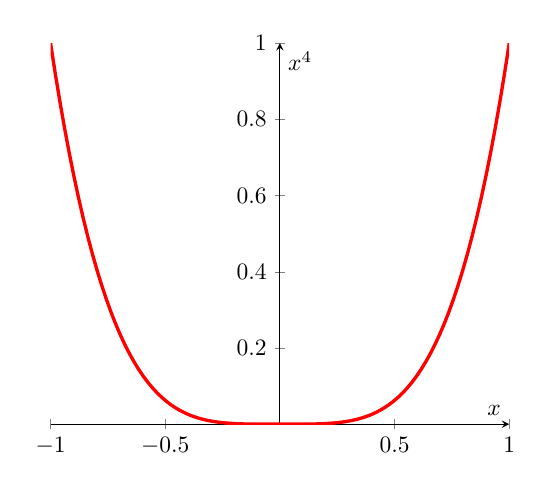
\begin{tikzpicture}[scale=0.85, transform shape]
\begin{axis}[axis lines = center, xlabel = \(x\), ylabel = \(x^4\)]
\addplot [domain=-1:1, samples=100, color=red, line width = 0.5mm]
{x^4};
\end{axis}
\end{tikzpicture} \\
\end{center}

Alternatively, we can say that $f'(x^*)=0$ and $f''(x^*) \geq 0$ or $f''(x^*)\leq 0$ is the necessary condition for determining whether $x^*$ is a maximum or minimum point.  

The following table summarizes the first and second-order conditions for local maximum and minimum. \\

\begin{tabularx}{\textwidth}{lXX}
\hline Condition & Maximum & Minimum \\
\hline \\ 
First-order necessary & $f^{\prime}(x)=0$ & $f^{\prime}(x)=0$ \\~\\
Second-order necessary ${ }^{\dagger}$ & $f^{\prime \prime}(x) \leq 0$ & $f^{\prime \prime}(x) \geq 0$ \\~\\
Second-order sufficient ${ }^{\dagger}$ & $f^{\prime \prime}(x)<0$ & $f^{\prime \prime}(x)>0$ \\~\\
\hline
\end{tabularx} \\
${ }^{\dagger}$ Applicable only after the first-order necessary condition has been satisfied.
\vspace{0.25em}

%%%%%%%%%%%% Conditions for Global Extrema

\subsection{Conditions for Global Extrema}
The conditions for global extrema are similar to those for local extrema, but now we need to look at the sign of $f''(x)$ over the entire domain of the function and not just locally at $x^*$. In particular, if $f''(x)<0$ for all $x$ in the domain of $f$, then any critical point of $f$ is a unique global maximum. This is because $f'(x)$ is decreasing over the entire domain of $x$, and can only be 0 at a unique critical point where it goes from positive to negative, implying that it is the unique global maximum. 

At this point, it is useful to define concave and convex functions. \\

\fbox{\begin{minipage}{\textwidth}
\begin{itemize}
  \item A function $f(x)$ is said to be \textit{concave} if  $ f''(x) \leq 0$ for all $x$.
  \item A function $f(x)$ is said to be \textit{convex} if  $ f''(x) \geq 0$ for all $x$.
\item A function $f(x)$ is said to be \textit{strictly concave} if  $ f''(x) < 0$ for all $x$.
  \item A function $f(x)$ is said to be \textit{strictly convex} if  $ f''(x) > 0$ for all $x$.
\end{itemize}
\end{minipage}} \\

So now, we can write the conditions for global extrema in terms of concave and convex functions. \\

\fbox{\begin{minipage}{\textwidth}
\begin{itemize}
  \item If a function is (strictly) concave, any critical point will give us a (unique) global maximum.
  \item If a function is (strictly) convex, any critical point will give us a (unique) global minimum.
\end{itemize}
\end{minipage}} \\

Since concave and convex functions allow flat regions, it is possible for there to be multiple extrema. This was the case in our example with $f(x)=2$, which is both a concave and a convex function as $f''(x)=0$. 

%%%%%%%%%%%%%%%%%%%%%%%%%%%%%%%%%%%%%%%%%%%%%%%%%%%%%%%%%%
% Unconstrained Optimization with Multiple Variables
%%%%%%%%%%%%%%%%%%%%%%%%%%%%%%%%%%%%%%%%%%%%%%%%%%%%%%%%%%

\section{Unconstrained Optimization with Multiple Variables}

In economics, we often encounter situations where we need to maximize a function that involves more than one variable. For example, we may want to determine the optimal quantity of two or more inputs, such as labor and capital, that a firm should use to produce a given level of output. 

To solve for the optimal values of multiple input variables, we need to take the partial derivative of the output function with respect to each input variable and set them equal to zero. This is the first-order condition (FOC) for multivariate functions. 

 For a function of two variables $f(x,y)$, the FOC is given by:
$$ f_x = \frac{\partial f}{\partial x} = 0 , \quad \quad f_y = \frac{\partial f}{\partial y} = 0 $$
Here, $f_x$ and $f_y$ are the partial derivatives of $f$ with respect to $x$ and $y$, respectively. In particular, $f_x$ captures, how $f$ changes as $x$ changes while holding $y$ constant. So when calculating the partial derivative with respect to one variable, we treat the other variable as a constant. \\

\textit{Example.} Let's find all the critical points for the function $$f(x,y) = x + y^2- x^2y$$ 
Note that, $f_x=1-2xy$ and $f_y = 2y-x^2$. 
Setting $f_x=0$, we get $xy=0.5$ and setting $f_y=0$, we get $y=0.5x^2$. 
Plugging $y=0.5x^2$ in  $xy=0.5$, we get at $x=1$ and $y=0.5$. So the critical point for this function is $(1,0.5)$. \\

\textit{Example.}  Consider the profit function $\pi(K,L) = Q(K,L) - rK - wL$, where $Q(K,L)$ is the production function that specifies the maximum quantity of output that can be produced using $K$ units of capital and $L$ units of labor. Here, $r$ and $w$ are the prices of capital and labor, respectively. 

The partial derivative of $\pi$ with respect to $L$ is given by:
 $$ \pi_L = \frac{\partial \pi}{\partial L}  = Q_L-w = 0   $$
Here, $Q_L$ is the partial derivative of the production function with respect to labor, which measures the marginal product of labor (MPL) or the increase in output resulting from an additional unit of labor. Similarly, $Q_K$ is the partial derivative of the production function with respect to capital, which measures the marginal product of capital (MPK). 

The partial derivative of $\pi$ with respect to $K$ is:
$$ \pi_K = \frac{\partial \pi}{\partial K}  = Q_K-r = 0   $$
At the critical point where both FOCs are satisfied, the firm will choose inputs so that the price of each input is equal to its marginal product. (Note that $Q_K$ and $Q_L$ are functions of $K$ and $L$.) \\

For multivariate functions, the second-order conditions involve calculating all the (own and cross) second partial derivatives of the function. We will skip details on these conditions here. However, it is important to note that the concept of concavity and convexity can be extended to multivariate functions. In particular, we can define a concave (convex) function as a function whose graph lies below (above) any line segment connecting any two points on the graph. (See the slides for Lecture 12 for more details.) Moreover, as before, any critical point of a multivariate (strictly) concave/convex function represents a (unique) global maximum/minimum. 

%%%%%%%%%%%%%%%%%%%%%%%%%%%%%%%%%%%%%%%%%%%%%%%%%%%%%%%%%%
% Constrained Optimization 
%%%%%%%%%%%%%%%%%%%%%%%%%%%%%%%%%%%%%%%%%%%%%%%%%%%%%%%%%%

\section{Constrained Optimization}
Lots of problems in economics involve optimizing a function subject to one or more constraints. For example, a firm may want to maximize its profits subject to production constraints, or a consumer may want to maximize their utility subject to a budget constraint. To solve such problems, we use the method of Lagrange multipliers. 

Suppose we want to maximize (or minimize) a function $f(x,y)$ subject to a constraint $g(x,y) = c$, where $c$ is a constant. The method of Lagrange multipliers involves constructing a new function, known as the Lagrangian, that combines the objective function and the constraint function as follows:
$$
L(x,y,\lambda)=f(x, y)+\lambda[c-g(x, y)]
$$

Here, $\lambda$ is the Lagrange multiplier. To find the optimal values of $x$ and $y$, we need to take partial derivatives of the Lagrangian with respect to each variable and the Lagrange multiplier and set them equal to zero. This gives us the first-order conditions:
\begin{align*}
L_x(x,y,\lambda) = \frac{\partial L}{\partial x} &= f_x(x, y)- \lambda \cdot g_x(x, y) = 0 \\
L_y(x,y,\lambda) = \frac{\partial L}{\partial y} &= f_x(x, y)- \lambda \cdot g_x(x, y) = 0 \\
L_{\lambda}(x,y,\lambda) = \frac{\partial L}{\partial \lambda} &= c-g(x, y) = 0 
\end{align*}
Here, $f_k$ and $g_k$ represent the partial derivative with respect to $x_k$ of the objective function and the constraint, respectively. 

Intuitively, the Lagrange multiplier method works because it allows us to take into account the constraint when optimizing the function. By introducing the Lagrange multiplier, we are effectively adding a penalty term to the objective function that accounts for the constraint. The Lagrange multiplier $\lambda$ has an economic interpretation as the shadow price of the constraint. It measures the change in the objective function resulting from a small change in the constraint function. Thus, the Lagrange multiplier provides us with information about the value of relaxing or tightening the constraint.\\


\textit{Example}. We want to maximize utility given by  $U(x,y) = x y$ subject to the budget constraint $4 x + y = 12$. 

We start by setting up the Lagrangian:
$$ L(x, y, \lambda) = x y + \lambda(12-4x-y) $$
First-order conditions:
\begin{align}
\frac{\partial L}{\partial x} &= y- 4 \lambda = 0  \\ 
\frac{\partial L}{\partial y} &= x- \lambda  = 0 \\ 
\frac{\partial L}{\partial \lambda} &= 12-4x-y = 0 
\end{align}
From equations (1) and (2), we have $y=4 \lambda$ and $x=\lambda$, which implies that $y=4x$. Plugging this in equation (3):
$$ 12-4x-4x = 0 \rightarrow x^* = 1.5, y^*=6, \lambda^* = 1.5 $$

Interpretation of $\lambda^*$: If income increases by a dollar, utility increases by $1.5$.\\

The method of Lagrange multipliers can be extended to problems with more than two variables and constraints. For example, consider the problem of maximizing a function $f(x,y,z)$ subject to two constraints $g(x,y,z) = c$ and $h(x,y,z) = m$, where $c$ and $m$ are constants. To solve this problem, we will need to introduce two Lagrange multipliers and then construct the Lagrangian function as follows:
$$L(x,y,z,\lambda,\mu) = f(x,y,z) + \lambda [c-g(x,y,z)] + \mu [m-h(x,y,z)]$$
To find the optimal values of $x$, $y$, and $z$ that maximize $f(x,y,z)$ subject to the two constraints, we can take the partial derivatives of the Lagrangian with respect to $x$, $y$, $z$, $\lambda$, and $\mu$, and set them equal to zero. 

\subsection*{Global Extrema with Constraints}

The Lagrange multiplier method transforms the constrained optimization problem of maximizing $f(x,y)$ subject to $g(x,y)$ into an unconstrained optimization problem of maximizing $ L(x, y, \lambda)$. We know that in the case of unconstrained optimization, any critical point of a concave function represents a global maximum. In the case of constrained optimization, if both $f(x,y)$ and $g(x,y)$ are concave, then $L(x,y,\lambda)$ will also be concave, and any critical point of $L(x,y,\lambda)$ will represent the global maximum of $f(x,y)$ subject to $g(x,y)$. However, requiring functions to be concave is a strong condition. We can instead use the weaker condition that $f(x,y)$ is quasiconcave, and the constraint set, $C=\{(x,y):g(x,y)=c\}$, is a convex set to ensure that we are identifying the global maximum. (See the slides for Lecture 12 for definitions.) \\

\fbox{\begin{minipage}{\textwidth}
The stationary point $(x_1^*, x_2^*, ..., x_n^*)$ of the Lagrangian corresponding to the problem of optimizing $f(x_1,x_2,..,x_n)$ subject to a constraint $g(x_1, x_2,...,x_n)=c$ is a global maximum if:
\begin{enumerate}
  \item $f(x_1,x_2,...,x_n)$ is quasiconcave
  \item The constraint set is convex\\
\end{enumerate}
\end{minipage}} \\


\section{Envelope Theorem}

In economics, we are often interested in understanding how the value of a function changes in response to certain \textit{parameters}. For example, we may be interested in how a consumer's utility changes in response to changes in prices, or how a firm's profits change in response to changes in wages. When analyzing how a function's value changes in response to changes in parameters, we need to consider both the direct impact of changing the parameters on the function's value, as well as the indirect impact of changing the parameters on the optimal inputs, which in turn affects the function's value. The Envelope Theorem tells us that we do not need to worry about the indirect effect of changing parameters on the optimal inputs --- we can simply focus on the direct effect. \\

\fbox{\begin{minipage}{\textwidth}
\textit{Envelope Theorem: Unconstrained Maximization} \\
Consider the following maximization problem: 
$$
\max_{x} \quad  f(x, \alpha)  
$$
Here, $\alpha$ is a parameter. Since the optimal input may depend on $\alpha$, let's denote it by $x^*(\alpha)$. Now let's define the \textit{maximum value function}:
$$ V(\alpha) = f(x^*(\alpha), \alpha) $$
The envelope theorem states that,
$$ V_{\alpha}= \frac{\partial V}{\partial \alpha} = f_{\alpha}^* $$
where $f_{\alpha}^*$ is the partial derivative of $f$ with respect to $x$ at $x^*$
\end{minipage}} \\

It is actually straightforward to see why this is the case. Note, that when we differentiate $V$ with respect to $\alpha$,
$$ V_{\alpha} = f_x^* \cdot \frac{\partial x^*}{\partial \alpha} + f_{\alpha}^* $$
Here, $f_x^*$ is the partial derivative of $f$ with respect to $x$ at $x^*$. By first order conditions for optimization, $f_x^*=0$, and hence $ V_{\alpha}=f_{\alpha}^* $. \\

\textit{Example.} Say we want to choose labor input $L$ to maximize profit $$\max_L \quad\pi(L, w) = \ln L-wL$$ 
Here, $w$ is the wage rate. Writing the first-order condition:
$$ \pi_L = \frac{1}{L}-w = 0 \rightarrow L^* = \frac{1}{w} $$
Since $L^*$ depends on $w$, we can write it as $L^*(w)$.

Now, we are interested in how optimal profit changes with respect to changes in wages. To answer this question, we first write down the maximum value function, which here depends on $w$. 
$$ V(w) = \pi(L^*(w), w) =  \ln L^*(w)-wL^*(w) $$
Now to see how $V(w)$ varies with $w$ we need the derivative of $V$ with respect to $w$. The envelope theorem says that this derivative is given by
$$ V'(w) =  \pi_w(L^*(w), w) =-L^*(w) = -\frac{1}{w}$$
We can also verify this by plugging in $L^*(w)=1/w$ in the expression for $V(w)$ and then differentiating with respect to $w$.
$$ V(w) =   \ln L^*(w)-wL^*(w) = \ln(1/w)-1 = \ln 1-\ln w-1 \rightarrow V'(w)=-\frac{1}{w}$$ 

The envelope theorem for constrained optimization problems is stated below. \\

\fbox{\begin{minipage}{\textwidth}
\textit{Envelope Theorem: Constrained Maximization} \\
Consider the following constrained optimization problem $$ \max_{x,y} \quad  f(x, y ; \alpha) \quad \text{s.t.} \quad G(x, y ; \alpha)=0$$ 
Lagrangian function:
$$
L(x,y,\lambda; \alpha) =f(x, y ; \alpha)+\lambda G(x, y ; \alpha)
$$
As before, define the value function $V(\alpha)=f(x^*, y^* ; \alpha)$. Then the envelope theorem states,
$$
\frac{\partial V}{\partial \alpha}=\frac{\partial L(x^*, y^*, \lambda^*; \alpha)}{\partial \alpha} $$
\end{minipage}} \\

The above theorem directly implies interpretation of the lagrange multiplier. Say max $f(x, y)$ subject to $g(x, y)=c$ 
Can think of the constraint as:
$$ G(x,y,c)= c-g(x,y) $$
So here $c$ is the parameter $\alpha$. Now what happens due to change in $c$ to the value function is given by 
$$
\frac{\partial V}{\partial \alpha}=\frac{\partial L(x^*, y^*, \lambda^*; \alpha)}{\partial \alpha} = \lambda^*$$ \\

\textit{Example}. We want to maximize the utility function $U(x_1,x_2)=x_1 x_2$ subject to the budget constraint $p_1 x_1 + p_2 x_2 = m$, where $m$ is the total income. We are interested in how the total utility changes due to a change in price of good 1. 

Setting up the Lagrangian: 
$$
L(x_1,x_2,\lambda) =x_1 x_2 + \lambda(m-p_1x_1-p_2x_2)
$$
First-order conditions:
\begin{align}
	L_{1} &= x_2-\lambda p_1=0 \\
	L_{2} &= x_1-\lambda p_2=0 \\
	L_{\lambda} &= m-p_1x_1-p_2x_2 = 0
\end{align}
Equations (4) and (5) imply that $x_2/x_1 = p_1/p_2$. Plugging $x_2 = p_1x_1/p_2$ in equation (6):
$$m-p_1x_1-p_2x_2 = m-p_1x_1-p_1x_1 \rightarrow x_1^*=\frac{m}{2p_1},x_2^*=\frac{m}{2p_2}, \lambda^* = \frac{m}{2p_1 p_2}  $$
Denote $L^*=L(x_1^*,x_2^*,\lambda^*)$. Then according to the envelope theorem how optimal utility changes with respect to $p_1$ is given by $$ \frac{\partial L^*}{\partial p_1} = -\lambda^* x_1^* = - \frac{m^2}{4p_1^2 p_2}$$

We can verify that this is true as:
$$ V(p_1,p_2,m) = x_1^* x_2^* = \frac{m^2}{4p_1 p_2} \rightarrow \frac{\partial V}{\partial p_1} = - \frac{m^2}{4p_1^2 p_2}$$

\end{document}